\ifx\wholebook\relax \else
% ------------------------

\documentclass[UTF8]{article}
%------------------- Other types of document example ------------------------
%
%\documentclass[twocolumn]{IEEEtran-new}
%\documentclass[12pt,twoside,draft]{IEEEtran}
%\documentstyle[9pt,twocolumn,technote,twoside]{IEEEtran}
%
%-----------------------------------------------------------------------------
%%
% loading packages
%
\newif\ifpdf
\ifx\pdfoutput\undefined % We're not running pdftex
  \pdffalse
\else
  \pdftrue
\fi
%
%
\ifpdf
  \RequirePackage[pdftex,%
            CJKbookmarks,%
       bookmarksnumbered,%
              colorlinks,%
          linkcolor=blue,%
              hyperindex,%
        plainpages=false,%
       pdfstartview=FitH]{hyperref}
\else
  \RequirePackage[dvipdfm,%
             CJKbookmarks,%
        bookmarksnumbered,%
               colorlinks,%
           linkcolor=blue,%
               hyperindex,%
         plainpages=false,%
        pdfstartview=FitH]{hyperref}
  \AtBeginDvi{\special{pdf:tounicode GBK-EUC-UCS2}} % GBK -> Unicode
\fi
\usepackage{hyperref}

% other packages
%-----------------------------------------------------------------------------
\usepackage{graphicx, color}
\usepackage{CJK}
%
% for programming 
%
\usepackage{verbatim}
\usepackage{listings}


\lstdefinelanguage{Smalltalk}{
  morekeywords={self,super,true,false,nil,thisContext}, % This is overkill
  morestring=[d]',
  morecomment=[s]{"}{"},
  alsoletter={\#:},
  escapechar={!},
  literate=
    {BANG}{!}1
    {UNDERSCORE}{\_}1
    {\\st}{Smalltalk}9 % convenience -- in case \st occurs in code
    % {'}{{\textquotesingle}}1 % replaced by upquote=true in \lstset
    {_}{{$\leftarrow$}}1
    {>>>}{{\sep}}1
    {^}{{$\uparrow$}}1
    {~}{{$\sim$}}1
    {-}{{\sf -\hspace{-0.13em}-}}1  % the goal is to make - the same width as +
    %{+}{\raisebox{0.08ex}{+}}1		% and to raise + off the baseline to match -
    {-->}{{\quad$\longrightarrow$\quad}}3
	, % Don't forget the comma at the end!
  tabsize=2
}[keywords,comments,strings]

\lstloadlanguages{C++, Lisp, Smalltalk}

% ======================================================================

\def\BibTeX{{\rm B\kern-.05em{\sc i\kern-.025em b}\kern-.08em
    T\kern-.1667em\lower.7ex\hbox{E}\kern-.125emX}}

\newtheorem{theorem}{Theorem}

%
% mathematics
%
\newcommand{\be}{\begin{equation}}
\newcommand{\ee}{\end{equation}}
\newcommand{\bmat}[1]{\left( \begin{array}{#1} }
\newcommand{\emat}{\end{array} \right) }
\newcommand{\VEC}[1]{\mbox{\boldmath $#1$}}

% numbered equation array
\newcommand{\bea}{\begin{eqnarray}}
\newcommand{\eea}{\end{eqnarray}}

% equation array not numbered
\newcommand{\bean}{\begin{eqnarray*}}
\newcommand{\eean}{\end{eqnarray*}}

\RequirePackage{CJK,CJKnumb,CJKulem,CJKpunct}
% we use CJK as default environment
\AtBeginDocument{\begin{CJK*}{GBK}{song}\CJKtilde\CJKindent\CJKcaption{GB}}
\AtEndDocument{\clearpage\end{CJK*}}

%
% loading packages
%

\RequirePackage{ifpdf}
\RequirePackage{ifxetex}

%
%
\ifpdf
  \RequirePackage[pdftex,%
       bookmarksnumbered,%
              colorlinks,%
          linkcolor=blue,%
              hyperindex,%
        plainpages=false,%
       pdfstartview=FitH]{hyperref}
\else\ifxetex
  \RequirePackage[bookmarksnumbered,%
               colorlinks,%
           linkcolor=blue,%
               hyperindex,%
         plainpages=false,%
        pdfstartview=FitH]{hyperref}
\else
  \RequirePackage[dvipdfm,%
        bookmarksnumbered,%
               colorlinks,%
           linkcolor=blue,%
               hyperindex,%
         plainpages=false,%
        pdfstartview=FitH]{hyperref}
\fi\fi
%\usepackage{hyperref}

% other packages
%--------------------------------------------------------------------------
\usepackage{graphicx, color}
\usepackage{subfig}
\usepackage{tikz}
\usetikzlibrary{matrix,positioning}

\usepackage{amsmath, amsthm, amssymb} % for math
\usepackage{exercise} % for exercise
\usepackage{import} % for nested input

%
% for programming
%
\usepackage{verbatim}
\usepackage{listings}
%\usepackage{algorithmic} %old version; we can use algorithmicx instead
\usepackage{algorithm}
\usepackage[noend]{algpseudocode} %for pseudo code, include algorithmicsx automatically
\usepackage{appendix}
\usepackage{makeidx} % for index support
\usepackage{titlesec}

\usepackage[cm-default]{fontspec}
\usepackage{xunicode}

% detect and select Chinese font
% ------------------------------
% the following cmd can list all availabe Chinese fonts in host.
% fc-list :lang=zh
\def\myfont{STHeiti}  % Under Mac OS X
\def\linuxfallback{WenQuanYi Micro Hei} % Under Linux
\def\winfallback{SimSun} % Under Windows
\suppressfontnotfounderror1 % Avoid setting exit code (error level) to break make process
\count255=\interactionmode
\batchmode
\font\foo="\myfont"\space at 10pt
\ifx\foo\nullfont
  \font\foo = "\linuxfallback"\space at 10pt
  \ifx\foo\nullfont
    \font\foo = "\winfallback"\space at 10pt
    \ifx\foo\nullfont
      \errorstopmode
      \errmessage{no suitable Chinese font found}
    \else
      \let\myfont=\winfallback % Windows
    \fi
  \else
    \let\myfont=\linuxfallback % Linux
  \fi
\fi
\interactionmode=\count255
\setmainfont[Mapping=tex-text]{\myfont}

\XeTeXlinebreaklocale "zh"  % to solve the line breaking issue
\XeTeXlinebreakskip = 0pt plus 1pt minus 0.1pt

\titleformat{\paragraph}
{\normalfont\normalsize\bfseries}{\theparagraph}{1em}{}
\titlespacing*{\paragraph}
{0pt}{3.25ex plus 1ex minus .2ex}{1.5ex plus .2ex}

\lstdefinelanguage{Smalltalk}{
  morekeywords={self,super,true,false,nil,thisContext}, % This is overkill
  morestring=[d]',
  morecomment=[s]{"}{"},
  alsoletter={\#:},
  escapechar={!},
  literate=
    {BANG}{!}1
    {UNDERSCORE}{\_}1
    {\\st}{Smalltalk}9 % convenience -- in case \st occurs in code
    % {'}{{\textquotesingle}}1 % replaced by upquote=true in \lstset
    {_}{{$\leftarrow$}}1
    {>>>}{{\sep}}1
    {^}{{$\uparrow$}}1
    {~}{{$\sim$}}1
    {-}{{\sf -\hspace{-0.13em}-}}1  % the goal is to make - the same width as +
    %{+}{\raisebox{0.08ex}{+}}1		% and to raise + off the baseline to match -
    {-->}{{\quad$\longrightarrow$\quad}}3
	, % Don't forget the comma at the end!
  tabsize=2
}[keywords,comments,strings]

% for better Haskell code outlook
\lstdefinelanguage{Haskell}{
  basicstyle=\small\ttfamily,
  flexiblecolumns=false,
  basewidth={0.5em,0.45em},
  literate={+}{{$+$}}1 {/}{{$/$}}1 {*}{{$*$}}1 {=}{{$=$}}1
           {>}{{$>$}}1 {<}{{$<$}}1 {\\}{{$\lambda$}}1
           {\\\\}{{\char`\\\char`\\}}1
           {->}{{$\rightarrow$}}2 {>=}{{$\geq$}}2 {<-}{{$\leftarrow$}}2
           {<=}{{$\leq$}}2 {=>}{{$\Rightarrow$}}2
           {\ .}{{$\circ$}}2 {\ .\ }{{$\circ$}}2
           {>>}{{>>}}2 {>>=}{{>>=}}2
           {|}{{$\mid$}}1
}[keywords,comments,strings]

\lstloadlanguages{C, C++, Lisp, Haskell, Python, Smalltalk}

\lstset{
  showstringspaces = false
}

% ======================================================================

\def\BibTeX{{\rm B\kern-.05em{\sc i\kern-.025em b}\kern-.08em
    T\kern-.1667em\lower.7ex\hbox{E}\kern-.125emX}}

%
% mathematics
%
\newcommand{\be}{\begin{equation}}
\newcommand{\ee}{\end{equation}}
\newcommand{\bmat}[1]{\left( \begin{array}{#1} }
\newcommand{\emat}{\end{array} \right) }
\newcommand{\VEC}[1]{\mbox{\boldmath $#1$}}

% numbered equation array
\newcommand{\bea}{\begin{eqnarray}}
\newcommand{\eea}{\end{eqnarray}}

% equation array not numbered
\newcommand{\bean}{\begin{eqnarray*}}
\newcommand{\eean}{\end{eqnarray*}}

\newtheorem{theorem}{Theorem}[section]
\newtheorem{lemma}[theorem]{Lemma}
\newtheorem{proposition}[theorem]{Proposition}
\newtheorem{corollary}[theorem]{Corollary}


\setcounter{page}{1}

\begin{document}

%--------------------------

% ================================================================
%                 COVER PAGE
% ================================================================

\title{插入排序的进化}

\author{刘新宇
\thanks{{\bfseries 刘新宇} \newline
  Email: liuxinyu95@gmail.com \newline}
  }

\maketitle
\fi

\markboth{插入排序}{初等算法}

\ifx\wholebook\relax
\chapter{插入排序的进化}
\numberwithin{Exercise}{chapter}
\fi

% ================================================================
%                 Introduction
% ================================================================
\section{简介}
\label{introduction} \index{插入排序}
上一章中,我们介绍了数据结构中的hello world——二叉搜索树。本章我们介绍排序算法中的hello world——插入排序\footnote{有人认为冒泡排序是最简单的排序算法。由于冒泡排序没有太大价值,本书并不介绍这一算法\cite{wiki-bubble-sort}。}。它很直观,但性能上不如一些分而治之的排序策略,如快速排序和归并排序。因此现代软件库中并不使用插入排序作为通用排序算法。我们将会分析插入排序性能上的问题,并且尝试逐步解决它们,最终进化到树排序。从而达到基于比较的排序算法的性能上限$O(n \lg n)$。同时,我们展示如何将hello world的数据结构和算法联系起来。

在扑克游戏的抓牌环节非常形像地描述了插入排序的思想\cite{CLRS}。考虑一副已经洗好的牌,然后我们开始一张一张的抓牌。

任何时候,我们手中的牌都是有序的。当我们抓到一张新牌的时候,我们按照牌的点数,把它插入到合适的位置。图\ref{fig:hand-of-cards}给出了这样一个例子。

\begin{figure}[htbp]
  \centering
  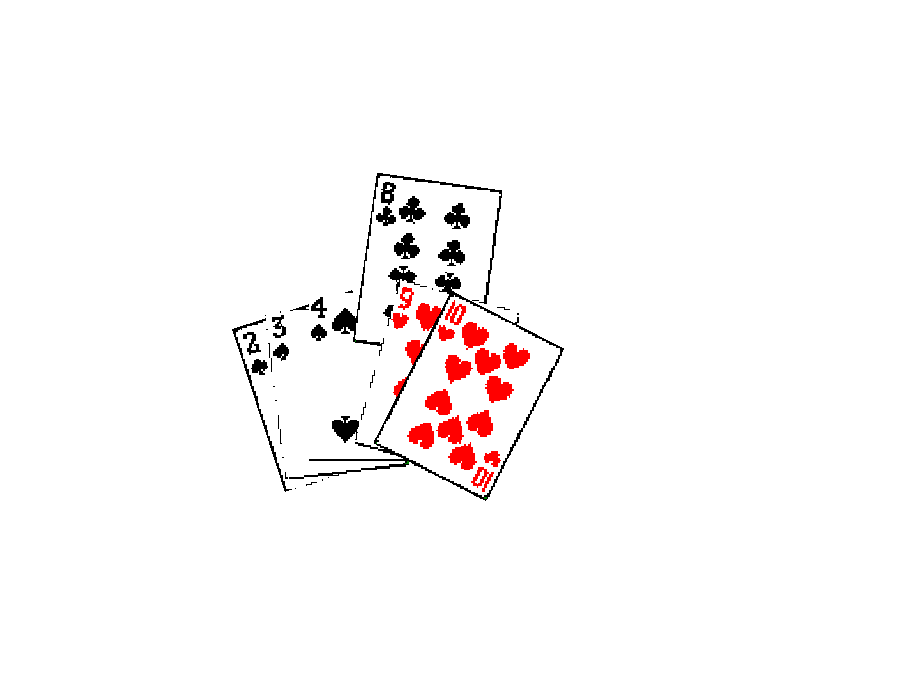
\includegraphics[scale=0.5]{img/hand-of-cards.eps}
  \caption{将草花8插入到一手牌中合适的位置。}
  \label{fig:hand-of-cards}
\end{figure}

根据这一思路,插入排序的算法可以这样给出:

\begin{algorithmic}
\Function{Sort}{$A$}
  \State $X \gets \phi$
  \For{each $x \in A$}
    \State \Call{Insert}{$X, x$}
  \EndFor
  \State \Return $X$
\EndFunction
\end{algorithmic}

我们在二叉搜索树一章曾经提到过folding的概念,插入排序也可以用这一概念来定义:

\be
  insert = foldL \quad insert \quad \phi
\ee

由于我们使用了$X$来存储排序结果,这一算法不是in-place排序算法。我们也可以把它改为in-place的。记待排序序列为$A = \{a_1, a_2, ... a_n\}$。

\begin{algorithmic}
\Function{Sort}{$A$}
  \For{$i \gets 2$ to $|A|$}
    \State insert $a_i$ to sorted sequence $\{a'_1, a'_2, ..., a'_{i-1} \}$
  \EndFor
\EndFunction
\end{algorithmic}

任何时候,当处理第$i$个元素的时候,所有$i$之前的元素都已经排好顺序了。我们不断将当前元素插入,直到处理完全部元素。这一过程如图\ref{fig:in-place-sort}所示。

\begin{figure}[htbp]
  \centering
  \includegraphics[scale=0.8]{img/in-place-sort.ps}
  \caption{左侧元素的顺序已经排好,不断将元素插入已序部份。}
  \label{fig:in-place-sort}
\end{figure}

这一过程中明显存在递归,因此可以表达为如下函数:

\be
sort(A) = \left \{
  \begin{array}
  {r@{\quad:\quad}l}
  \phi & A = \phi \\
  insert(sort(\{a_2, a_3, ...\}), a_1) & otherwise
  \end{array}
\right.
\ee

% ================================================================
% Insertion
% ================================================================
\section{插入}
\index{插入排序!插入}

我们尚未回答如何进行插入。人们还无法确切知道,大脑是如何在一手牌中快速找到插入位置的。

使用计算机,我们可以通过扫描找到插入位置。扫描时可以从左向右或者从右向左。但如果序列是用数组存储的,就必须从右向左进行扫描。

\begin{algorithmic}
\Function{Sort}{$A$}
  \For{$i \gets 2$ to $|A|$}
    \Comment{Insert $A[i]$ to sorted sequence $A[1...i-1]$}
    \State $x \gets A[i]$
    \State $j \gets i-1$
    \While{$j > 0 \land x < A[j]$ }
      \State $A[j+1] \gets A[j]$
      \State $j \gets j - 1$
    \EndWhile
    \State $A[j+1] \gets x$
  \EndFor
\EndFunction
\end{algorithmic}

有读者认为从左向右更加自然,但是这样性能上会出现问题。实际上,在数组中的任意位置插入元素是一个比较费时的操作。由于数组是连续存储元素的,如果需要在第$i$个位置插入元素$x$,我们需要把所有$i$后面的元素,包括第$i+1$、第$i+2$……都向右移动(shift)。之后,第$i$个位置才能空出来用以插入$x$。图\ref{fig:array-shift}描述了这一过程。

\begin{figure}[htbp]
  \centering
  \includegraphics[scale=0.7]{img/array-shift.ps}
  \caption{将元素$x$插入数组$A$中的第$i$个位置。}
  \label{fig:array-shift}
\end{figure}

从左向右扫描时,如果数组的长度为$n$,我们需要扫描前面$i$个元素,然后进行$n-i+1$次移动,最后将$x$插入到第$i$个位置。也就是说,从左向右扫描会遍历整个数组。相反,如果从右向左扫描,我们最多只需要检察$i$个元素,并且随着扫描将它们向右移动。

下面的Python例子程序实现了上述算法。

\lstset{language=Python}
\begin{lstlisting}
def isort(xs):
    n = len(xs)
    for i in range(1, n):
        x = xs[i]
        j = i - 1
        while j >= 0 and x < xs[j]:
            xs[j+1] = xs[j]
            j = j - 1
        xs[j+1] = x
\end{lstlisting}

这一实现也存在一些变形,例如下面的ANSI C语言的例子程序。但是它比我们给出的插入方法的操作次数多一些。

\lstset{language=C}
\begin{lstlisting}
void isort(Key* xs, int n){
  int i, j;
  for(i=1; i<n; ++i)
    for(j=i-1; j>=0 && xs[j+1] < xs[j]; --j)
      swap(xs, j, j+1);
}
\end{lstlisting}

这是因为交换函数\texttt{swap}通常使用一个中间变量来实现,如下:

\begin{lstlisting}
void swap(Key* xs, int i, int j){
  Key temp = xs[i];
  xs[i] = xs[j];
  xs[j] = temp;
}
\end{lstlisting}

若内循环的次数为$m$,上述ANSI C程序总共需要$3m$次赋值操作,而我们给出的算法及其Python实现使用shift来代替swap,它只需要$m+2$次赋值操作。

我们也可以提供单独的\textproc{Insert}()函数,然后在插入算法中调用它。我们略过这些实现细节,读者可以作为练习尝试这些不同的实现。

尽管有这些实现上的差异,从左向右也好,从右向左也好,所有这些插入算法的复杂度都是$O(n)$的,其中$n$为序列的长度。因此插入排序的总体复杂度为$O(n^2)$。

\begin{Exercise}

\begin{itemize}
\item 定义单独的插入函数,并在通用的插入排序算法中调用它。请尝试用命令式的方式和函数式的方式给出不同的实现。
\end{itemize}

\end{Exercise}

% ================================================================
% Improvement 1
% ================================================================

\section{改进一}
\index{插入排序!二分查找}

人的大脑是如何快速在一手牌中找到插入位置的?似乎不是逐一扫描。任何时刻,我们手中的牌都是已序的,因此我们可以用二分查找来搜索插入位置。

我们将来后面的章节中专门详细讨论搜索算法。本节仅仅对二分查找做一个简单介绍。

下面的排序算法改为调用二分查找来确定插入的位置:

\begin{algorithmic}
\Function{Sort}{$A$}
  \For{$i \gets 2$ to $|A|$}
    \State $x \gets A[i]$
    \State $p \gets $ \Call{Binary-Search}{$A[1...i-1], x$}
    \For{$j \gets i$ down to $p$}
      \State $A[j] \gets A[j-1]$
    \EndFor
    \State $A[p] \gets x$
  \EndFor
\EndFunction
\end{algorithmic}

我们不再逐一扫描元素,考虑数组中的片断$\{A[1], ..., A[i-1] \}$已经有序了。假设它们是单调增的,我们需要找到一个位置$j$使得$A[j-1] \leq x \leq A[j]$。我们可以先检查中间的元素$A[\lfloor i/2 \rfloor]$。如果$x$比它小,我们需要接下来递归地在前一半序列进行二分查找;否则我们需要查找后一半序列。

由于我们每次都排除掉一半元素,所以这一过程需要$O(\lg n)$的时间来找到插入的位置。

\begin{algorithmic}
\Function{Binary-Search}{$A, x$}
  \State $l \gets 1$
  \State $u \gets 1+|A|$
  \While{$l < u$}
    \State $m \gets \lfloor \frac{l+u}{2} \rfloor$
    \If{$A[m] = x$}
      \State \Return $m$ \Comment{Find a duplicated element}
    \ElsIf{$A[m] < x$}
      \State $l \gets m+1$
    \Else
      \State $u \gets m$
    \EndIf
  \EndWhile
  \State \Return $l$
\EndFunction
\end{algorithmic}

这一改进并不能提高插入排序的复杂度,结果仍然是$O(n^2)$。此前的算法进行了$O(n^2)$次比较和$O(n^2)$次移动,使用二分查找后,比较次数变成了$O(n \lg n)$,但是移动次数还是$O(n^2)$。

下面的Python例子程序实现了这一改进。

\lstset{language=Python}
\begin{lstlisting}
def isort(xs):
    n = len(xs)
    for i in range(1, n):
        x = xs[i]
        p = binary_search(xs[:i], x)
        for j in range(i, p, -1):
            xs[j] = xs[j-1]
        xs[p] = x

def binary_search(xs, x):
    l = 0
    u = len(xs)
    while l < u:
        m = (l+u)/2
        if xs[m] == x:
            return m
        elif xs[m] < x:
            l = m + 1
        else:
            u = m
    return l
\end{lstlisting}

\begin{Exercise}
使用递归来实现二分查找。编程语言不必限定为函数式的。
\end{Exercise}

% ================================================================
% Improvement 2
% ================================================================

\section{改进二}
\index{插入排序!链表插入排序}

虽然我们通过二分查找,将搜索插入位置的时间降低为$O(n \lg n)$,但是移动元素的时间仍然是$O(n^2)$的。由于序列是使用数组存储的,因此我们无法避免这个耗时的操作。数组在内存中连续存储元素,插入操作必然需要通过连续的移动已空出位置。我们也可以尝试使用链表来表达序列,这样插入操作就可以由线性时间$O(n)$提高到常数时间$O(1)$。

\be
  insert(A, x) = \left \{
  \begin{array}
  {r@{\quad:\quad}l}
  \{ x \} & A = \phi \\
  \{ x \} \cup A & x < a_1 \\
  \{ a_1 \} \cup insert(\{ a_2, a_3, ... a_n\}, x)& otherwise
  \end{array}
\right.
\ee

这一算法可以翻译为下面的Haskell例子程序。

\lstset{language=Haskell}
\begin{lstlisting}
insert [] x = [x]
insert (y:ys) x = if x < y then x:y:ys else y:insert ys x
\end{lstlisting}

本章开头部份给出的插入排序定义,可以通过调用这一函数来完成。

\begin{lstlisting}
isort [] = []
isort (x:xs) = insert (isort xs) x
\end{lstlisting}

也可以用folding来实现:

\begin{lstlisting}
isort = foldl insert []
\end{lstlisting}

也可以用imperative的方式实现链表的插入排序。令函数\textproc{Key}($x$)返回链表节点$x$存储的元素,函数\textproc{Next}($x$)用以访问链表中的下一个节点。

\begin{algorithmic}
\Function{Insert}{$L, x$}
  \State $p \gets$ NIL
  \State $H \gets L$
  \While{$L \neq$ NIL $\land $ \Call{Key}{$L$} $<$ \Call{Key}{$x$}}
    \State $p \gets L$
    \State $L \gets $ \Call{Next}{$L$}
  \EndWhile
  \State \Call{Next}{$x$} $\gets L$
  \If{$p \neq$ NIL}
    \State $H \gets x$
  \Else
    \State \Call{Next}{$p$} $\gets x$
  \EndIf
  \State \Return $H$
\EndFunction
\end{algorithmic}

下面的ANSI C例子代码定义了链表的节点:

\lstset{language=C}
\begin{lstlisting}
struct node{
  Key key;
  struct node* next;
};
\end{lstlisting}

根据此定义,插入程序可以实现如下:

\begin{lstlisting}
struct node* insert(struct node* lst, struct node* x){
  struct node *p, *head;
  p = NULL;
  for(head = lst; lst && x->key > lst->key; lst = lst->next)
    p = lst;
  x->next = lst;
  if(!p)
    return x;
  p->next = x;
  return head;
}
\end{lstlisting}

我们也可以不用基于指针或者引用的数据结构,而通过另一个索引数组来实现链表。对于任何数组元素$A[i]$,$Next[i]$保存了$A[i]$下一个元素的索引。也就是说$A[Next[i]]$是$A[i]$的下一个元素。

利用这种索引链表的插入算法可以定义如下:

\begin{algorithmic}
\Function{Insert}{$A, Next, i$}
  \State $j \gets \perp$
  \While{$Next[j] \neq$ NIL $\land A[Next[j]] < A[i]$}
    \State $j \gets Next[j]$
  \EndWhile
  \State $Next[i] \gets Next[j]$
  \State $Next[j] \gets i$
\EndFunction
\end{algorithmic}

其中$\perp$表示索引表$Next$的头部。下面的Python例子程序实现了使用这种形式链表的插入排序算法。

\lstset{language=Python}
\begin{lstlisting}
def isort(xs):
    n = len(xs)
    next = [-1]*(n+1)
    for i in range(n):
        insert(xs, next, i)
    return next

def insert(xs, next, i):
    j = -1
    while next[j] != -1 and xs[next[j]] < xs[i]:
        j = next[j]
    next[j], next[i] = i, next[j]
\end{lstlisting}

虽然使用链表后,插入操作降低为常数时间。但是我们只能遍历链表来找到合适的插入位置。因此算法需要进行$O(n^2)$次比较。与数组不同,链表不支持随机访问(random access),我们不能利用二分查找在链表中搜索插入位置。

\begin{Exercise}
\begin{itemize}
\item 选择一种imperative编程语言,实现完整的链表插入排序算法。
\item 使用索引数组的链表,排序结果是一个重新排列的索引。给出一个方法,根据新的索引,重新排列数组元素。
\end{itemize}
\end{Exercise}

% ================================================================
% Final improvement
% ================================================================

\section{使用二叉搜索树的最终改进}
\index{插入排序!二叉搜索树}

我们似乎钻进了死胡同:必须同时提高查找的速度和插入的速度,单独提高其中的一个仍然会保持$O(n^2)$的复杂度。

我们必须使用二分查找,这是唯一能把比较次数降低到$O(\lg n)$的方法。另一方面,我们必须改变数据结构,因为我们不能在普通数组中实现常数时间的插入。

这使我们想到了hello world数据结构―二叉搜索树。它本身就被定义为支持二分查找。同时,一旦找到了插入的位置,我们可以在常数$O(1)$时间插入一个新节点。

于是,我们最终获得了下面的算法:

\begin{algorithmic}
\Function{Sort}{$A$}
  \State $T \gets \phi$
  \For{each $x \in A$}
    \State $T \gets $ \Call{Insert-Tree}{$T, x$}
  \EndFor
  \State \Return \Call{To-List}{$T$}
\EndFunction
\end{algorithmic}

其中函数\textproc{Insert-Tree}()和\textproc{To-List}()的定义在上一章。

根据我们对二叉搜索树的分析,树排序的性能为$O(n \lg n)$,这达到了基于比较的排序算法的时间下限\cite{Knuth}。

\section{Short summary}
In this chapter, we present the evolution process of insertion sort. Insertion
sort is well explained in most textbooks as the first sorting algorithm.
It has simple and straightforward idea, but the performance is quadratic.
Some textbooks stop here, but we want to show that there exist ways to improve
it by different point of view. We first try to save the comparison time
by using binary search, and then try to save the insertion operation by
changing the data structure to linked-list. Finally, we combine these
two ideas and evolute insertion sort to tree sort.

\begin{thebibliography}{99}

\bibitem{wiki-bubble-sort}
http://en.wikipedia.org/wiki/Bubble\_sort

\bibitem{CLRS}
Thomas H. Cormen, Charles E. Leiserson, Ronald L. Rivest and Clifford Stein.
``Introduction to Algorithms, Second Edition''. ISBN:0262032937. The MIT Press. 2001

\bibitem{Knuth}
Donald E. Knuth. ``The Art of Computer Programming, Volume 3: Sorting and Searching (2nd Edition)''. Addison-Wesley Professional; 2 edition (May 4, 1998) ISBN-10: 0201896850 ISBN-13: 978-0201896855

\end{thebibliography}

\ifx\wholebook\relax\else
\end{document}
\fi
